\chapter{Literature Review}
This chapter systematically reviews the existing research on DTN and its application to email services. The chapter begins by outlining the fundamental characteristics of interplanetary network environments and analyzing the inherent limitations of the traditional TCP/IP protocol suite in this context, thereby establishing the necessity of the DTN paradigm. It then delves into the core mechanisms and layered architecture of DTN.

Building on this foundation, the focus shifts to a specific application scenario: email. An analysis is presented on how the conversational nature of the Simple Mail Transfer Protocol (SMTP) conflicts with the operational principles of DTN environments. Subsequently, this chapter examines the prevailing gateway-based solutions that integrate DTN with conventional TCP/IP networks. This includes a detailed analysis of key IETF drafts, such as Johnson Draft~\cite{draft-johnson-dtn-interplanetary-smtp} which defines the service, draft-blanchet-dtn-email-over-bpas~\cite{draft-blanchet-dtn-email-over-bp} which specifies the data encapsulation format, and a corresponding draft for Domain Name System (DNS)~\cite{draft-johnson-dtn-interplanetary-dns} that addresses critical service dependencies. Finally, the chapter introduces BPMail~\cite{bpmail}, a key open-source implementation of this concept, and summarizes the current state of research to identify existing limitations. This provides the theoretical basis for the objectives and contributions of this dissertation.

\section{Characteristics of Interplanetary Networks}
Interplanetary Network environments differ fundamentally from the terrestrial internet, primarily in the following aspects:


\begin{enumerate}
  \item Long Delays
  
  Due to the vast distances involved, signal propagation between celestial bodies can introduce noticeable delays. For instance, light-speed communication between Earth and Moon takes about 1.3 seconds each way.

  \item Frequent Disruptions
  
  Communication links are often unavailable for hours or even days due to factors such as celestial occlusion (e.g., planets rotating to block the line of sight) and the continuous orbital motion of satellites.

  \item Asymmetric Channel Bandwidth
  
  The uplink bandwidth from Earth to deep space is typically much higher than the downlink bandwidth from deep space back to Earth.

  \item High Bit Error Rates (BER)
  
  Space radiation and long-distance signal degradation result in significantly higher data transmission error rates compared to terrestrial channels like fiber optics.
\end{enumerate}

The traditional TCP/IP protocol suite was designed for the low-latency, high-stability terrestrial Internet. Its core assumption of a persistent, end-to-end connection is violated in interplanetary environments, leading to its failure. Key limitations include connection establishment failures, the breakdown of ``chatty'' protocols, and the misinterpretation of disruptions as network congestion~\cite{sarkar2011survey}. Consequently, a fundamentally new network architecture is required.

\section{DTN Architecture}

To address these challenges, Vint Cerf and colleagues proposed Delay-Tolerant Networking (DTN). DTN eliminates the dependency on real-time, end-to-end paths by employing the Bundle Protocol (BP)~\cite{rfc9171}, the ``store-carry-forward'' mechanism, and the optional Custody Transfer feature, enabling reliable communication in space network environments. Typically implemented shown in Figure \ref{Typicall_DTN_implementation} as an overlay network positioned between the application and transport layers, DTN operates in conjunction with diverse underlying network technologies through Convergence Layer Adapters.
\begin{figure}[h]
    \centering
    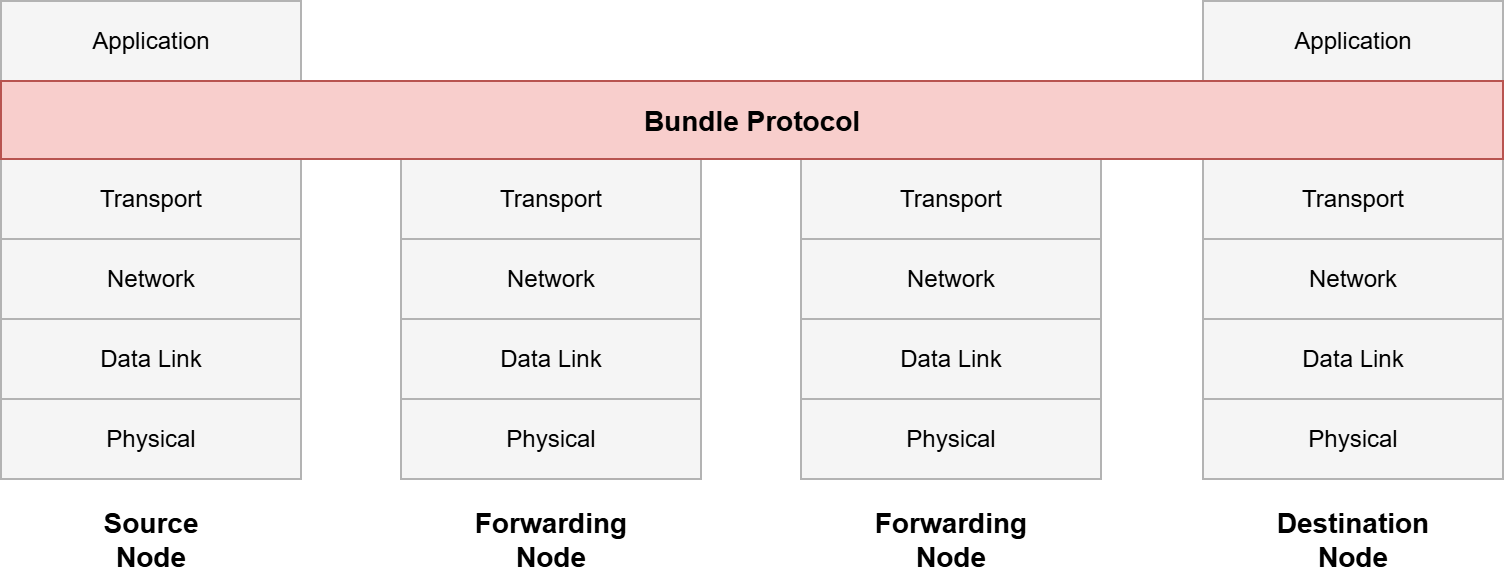
\includegraphics[width=\linewidth]{Literature Review/Typicall_DTN_implementation.png}
    \caption{Typicall DTN implementation}
    \label{Typicall_DTN_implementation}
\end{figure}

\section{Email System Architecture}

The traditional email system is a classic example of a distributed, store-and-forward system. It relies on a set of logical components and standardized protocols working in concert to enable global message delivery.

\subsection{Core Components}

\begin{figure}[h]
    \centering
    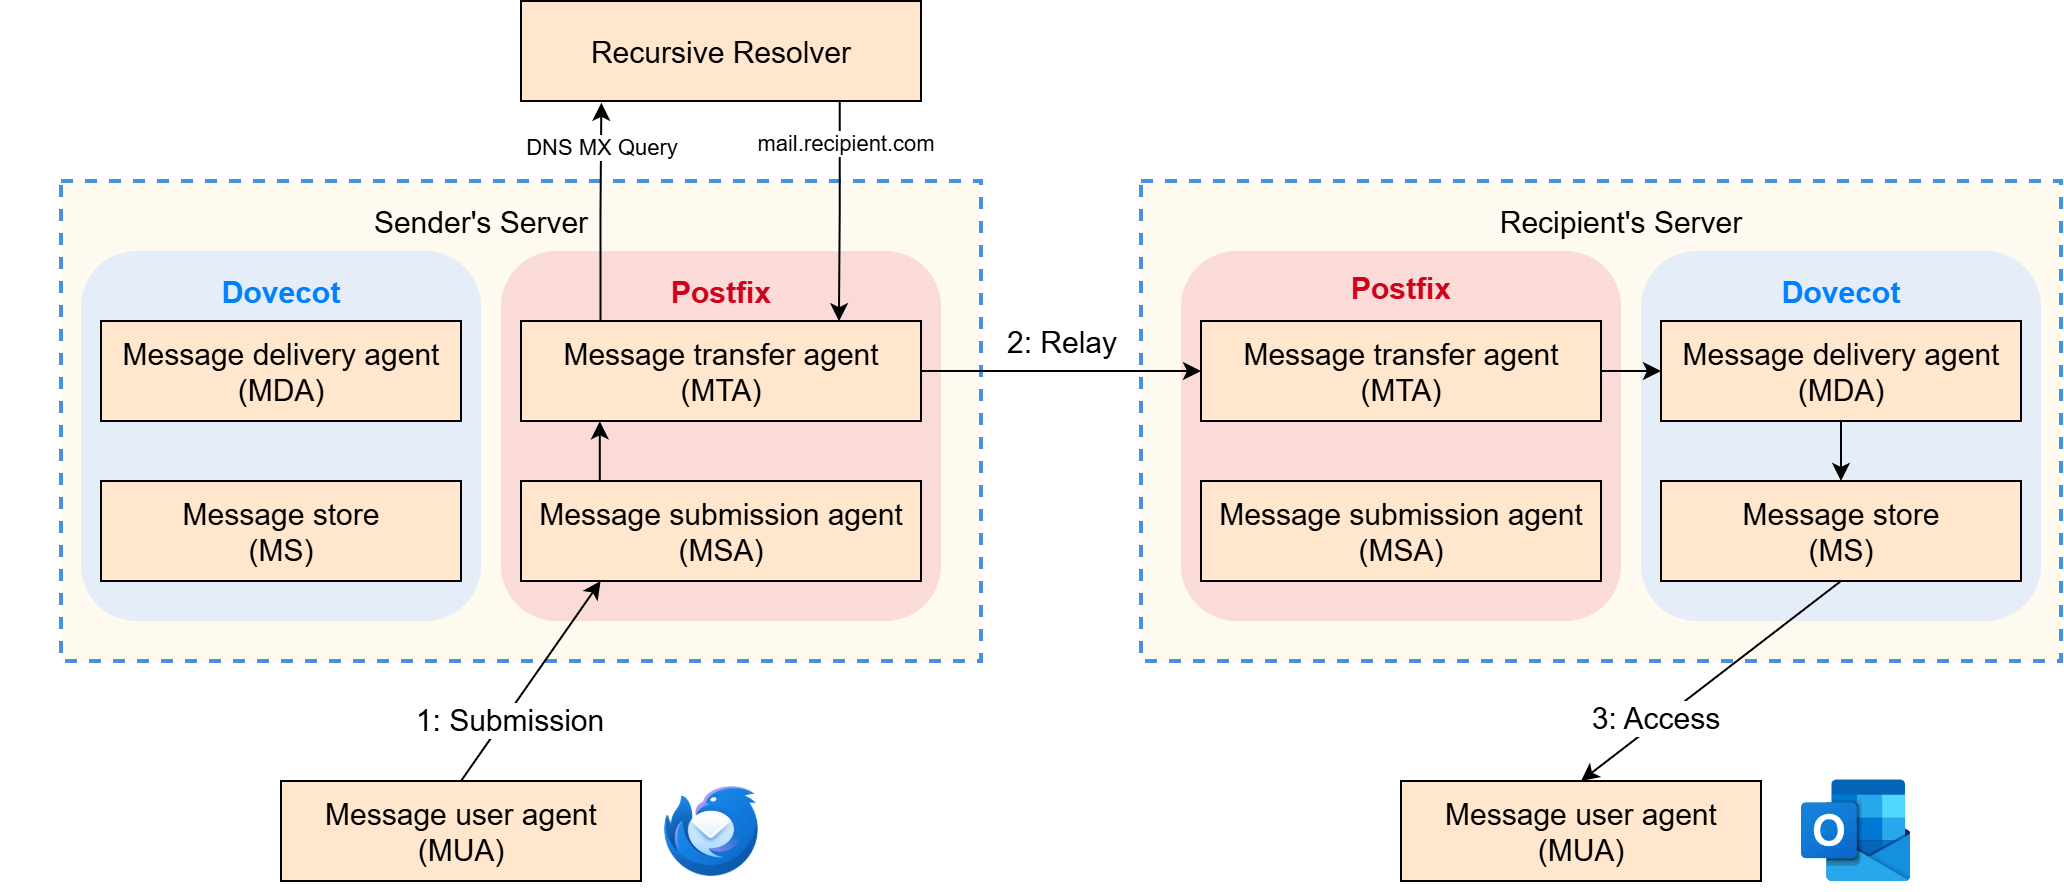
\includegraphics[width=\linewidth]{Literature Review/Email_architecture.png}
    \caption{Email architecture}
    \label{Email_architecture}
\end{figure}
As shown in Figure \ref{Email_architecture}, a typical email transaction involves the following core components~\cite{rfc5598}:

\begin{enumerate}
    \item Mail User Agent (MUA): This is the client software with which the user directly interacts, such as Mozilla Thunderbird or Microsoft Outlook. The MUA is responsible for composing, displaying, and managing emails, and it communicates with mail servers using standard protocols.
    \item Mail Submission Agent (MSA): The MUA submits an outgoing email to an MSA. The MSA authenticates the user, performs a preliminary check of the message format, and then passes the email to a Mail Transfer Agent (MTA). Typically, MSA functionality is provided by MTA software (e.g., Postfix) on a dedicated port (port 587).
    \item Mail Transfer Agent (MTA): The MTA is the central hub of the email system, acting as a ``post office.'' Examples include Postfix and Sendmail. Its primary responsibility is to relay emails from one server to another. It does this by looking up the Mail Exchange (MX) record in the DNS for the recipient's domain to find the next-hop MTA and then uses SMTP to forward the message.
    \item Mail Delivery Agent (MDA): When an email arrives at its final destination MTA, an MDA takes over. The MDA is responsible for placing the email into the appropriate user's mailbox. Software like Dovecot provides robust MDA functionality, including the ability to filter and sort incoming messages.
    \item Message Store: This is the physical or logical location on the server where emails are stored, representing the final, static destination in an email's lifecycle. It is a passive component, written to by the MDA and read from by the IMAP/POP3 server in response to MUA requests. The two most common storage formats are~\cite{MaildirSpec}:
    \begin{enumerate}
        \item mbox: Stores all of a user's emails concatenated into a single file. While simple to implement, this format suffers from performance issues with concurrent access and can pose challenges for data recovery.
        \item Maildir: Creates a separate file for each email, organized within a specific directory structure (e.g., cur, new, tmp). This format avoids file-locking issues, is more robust, and is the preferred choice in modern mail systems.
    \end{enumerate}
\end{enumerate}

\subsection{Key Protocols}

Communication between the components described above relies on the following key protocols:

\begin{enumerate}
  \item SMTP (Simple Mail Transfer Protocol)

  SMTP~\cite{rfc5321} is the standard protocol for sending and relaying email. It is a TCP-based, text-driven ``push'' protocol characterized by its highly conversational or interactive nature. A successful mail transfer involves a sequence of strictly ordered command-and-response interactions between client and server, such as: \texttt{EHLO/HELO} (greeting and identification), \texttt{AUTH} (authentication), \texttt{MAIL FROM} (sender's address), \texttt{RCPT TO} (recipient address), \texttt{DATA} (start of message content), and \texttt{QUIT} (termination). After each command, the client must wait for a three-digit status code (e.g., 250 OK) from the server before proceeding. This tightly coupled model requires low latency and stable network connections.
  \item POP3 (Post Office Protocol 3) / IMAP (Internet Message Access Protocol)

  These protocols are used by an MUA to retrieve and manage emails from a server. POP3~\cite{rfc1939} is a simple ``pull'' protocol that usually downloads all messages to the local client and deletes them from the server. IMAP~\cite{rfc9051} is more flexible, allowing server-side folder management and message status synchronization across multiple clients, with messages typically remaining stored on the server.

  \item TCP (Transmission Control Protocol)

  All of the above application protocols run over TCP, which strongly influence email system behavior and performance. TCP establishes a connection via a three-way handshake and guarantees in-order, lossless delivery using acknowledgments, retransmissions, and congestion control. These mechanisms introduce additional round trips beyond the application’s own command/response exchanges, making end-to-end latency directly visible to SMTP, POP3, and IMAP. Specifically: (a) connection setup/teardown incur RTT-dependent delays; (b) per-command turn-taking in SMTP/POP3/IMAP is serialized atop TCP’s flow, so each application step often waits at least one RTT; (c) TCP’s slow start and congestion control limit initial throughput and reduce the congestion window on loss, which can stall or stretch message transfers; (d) head-of-line blocking within a single TCP stream means that any lost segment pauses delivery of subsequent bytes, amplifying the impact of even modest packet loss when RTT is large. As a result, email protocols—especially SMTP’s highly interactive exchange and IMAP’s metadata-rich operations—perform best on low-latency, low-loss paths, while high RTT or intermittent loss can significantly degrade responsiveness, prolong sessions, and increase timeout/retry behavior.

  \item Anti-Spam and Authentication Mechanisms (via DNS Queries)

  To combat spam and phishing, a suite of protocols works alongside SMTP to verify sender identity. These protocols do not transfer message data themselves but leverage the DNS to publish and check authentication policies. 
  \begin{itemize}
    \item DNSBL (Domain Name System blocklist) check occurs the moment a sender's MTA connects, even before significant SMTP commands are exchanged. The recipient's MTA queries a DNS-based, real-time database of IP addresses known for sending spam. If the connecting IP is listed, the MTA can reject the connection outright.
    \item SPF (Sender Policy Framework) allows a domain to specify which MTAs are authorized to send email on its behalf. The recipient's MTA checks the IP address of the sender's MTA against this authorized list published in the domain’s DNS records. 
    \item DKIM (DomainKeys Identified Mail) provides message integrity by adding a digital signature to the email. The sender's MTA signs the message with a private key, and the recipient's MTA uses a corresponding public key from the DNS to verify that the message is authentic and has not been altered in transit. 
    \item DMARC (Domain-based Message Authentication, Reporting, and Conformance) unifies SPF and DKIM. It allows the sender's domain to set a policy that instructs the recipient's MTA on how to handle messages that fail these checks (e.g., to quarantine or reject them) and provides a reporting mechanism for monitoring.
  \end{itemize}
\end{enumerate}

In summary, the traditional email system is a complex ecosystem of components and interactive protocols. Its operation depends on the assumption of a low-latency and continuously available underlying network—namely, the TCP/IP-based Internet. This assumption makes it unsuitable for DTN.

\section{Solutions for DTN Email}
To adapt traditional email systems for DTN environments, a series of collaborative IETF drafts has been proposed. Together, they define a comprehensive solution by addressing three key aspects: service interaction, data format, and dependency resolution.

\subsection{Service Interaction}

Johnson Draft \cite{draft-johnson-dtn-interplanetary-smtp} proposes a solution centered on an SMTP gateway. Its core concept is to place a gateway between the DTN and a traditional TCP/IP network. This gateway acts as a protocol translator, converting TCP-based SMTP sessions into BP transmissions for outgoing mail, and reversing the process for incoming mail. This approach enables seamless integration between legacy mail servers and a DTN. The detailed workflow is as follows:

\begin{enumerate}
    \item \textit{Terminate SMTP Session}
    
    The gateway presents itself as a standard SMTP server to the local mail server (e.g., Postfix). When the local server attempts to send an email to a destination within the DTN, it establishes a standard SMTP connection with the gateway.
    \item \textit{Package Mail Transaction}
    
    The gateway engages in and completes the entire SMTP conversation, collecting all necessary information, including the sender, recipient(s), and the full message header and body.
    \item \textit{Trigger Bundle Encapsulation}
    
    The gateway then takes the complete mail transaction and triggers its encapsulation into one or more BP bundles, which are then dispatched into the DTN.
\end{enumerate}

This scheme provides excellent backward compatibility with existing email infrastructure. It effectively answers the question of how to interface with the DTN, but it does not specify the precise internal format of the encapsulated bundle.

\subsection{Data Format}

To complement and complete the gateway solution, the Blanchet Draft \cite{draft-blanchet-dtn-email-over-bp} was introduced. Rather than being a competing proposal, this draft provides a detailed technical specification for how an email should be encapsulated within a bundle, defining a standard format. Its key contributions include:

\begin{itemize}
    \item \textit{Data Model}
    
    Specifies how a standard email message (compliant with RFC 5322) should be mapped into a BP bundle.
    \item \textit{Block Definition}
    
    Recommends that the entire email, including headers and body, be placed either in the bundle's primary payload block or in a separate payload block.
    \item \textit{Metadata Mapping}
    
    Explores the possibility of mapping key email header fields (such as the Message-ID) to bundle metadata to facilitate more efficient processing.
\end{itemize}

Thus, these two drafts are complementary: the Johnson draft defines \textit{what} the gateway does (interacts with the SMTP world), while the Blanchet draft defines \textit{how} the gateway does it (generates a standardized email bundle). A complete, standards-compliant gateway implementation should adhere to both.

\subsection{Dependencies Resolution}

Email routing is critically dependent on DNS for resolving MX records. Standard DNS, however, is unworkable in a DTN environment. The Johnson DNS Draft \cite{draft-johnson-dtn-interplanetary-dns} addresses this crucial dependency by proposing a DTN-DNS gateway. This gateway intercepts local DNS queries, packages them into bundles for transmission across the DTN to an authoritative server, and returns the response, also in a bundle. This mechanism is fundamental to ensuring that the DTN email system can correctly route messages.

\section{The BPMail Gateway}

The value of theoretical drafts lies in their practical feasibility. The ASCENT project \cite{bpmail}, initiated by California State University, developed an open-source tool called BPMail, which is a concrete implementation of the gateway concept. BPMail is designed to integrate with the Postfix mail system as a custom mail delivery agent.

BPMail's workflow aligns closely with the behavior described in the Johnson draft. It is invoked by Postfix, receives a complete email message, and then uses the library functions of ION-DTN (a leading DTN protocol stack developed by NASA) to encapsulate the email into a bundle and inject it into the local ION node. BPMail provides practical validation for the theoretical proposals, and its encapsulation process represents the core operation that the Blanchet Draft aims to standardize. Therefore, BPMail serves as an ideal tool for researching and simulating a complete DTN email system based on this series of drafts.

\section{Summary}

In summary, the existing literature has established a clear and collaborative technical framework for enabling email communication in DTN environments. The technology roadmap, from the analysis of space network requirements to the development of the DTN architecture and a series of complementary standardization drafts, is well-defined. The existence of practical tools like BPMail further demonstrates the framework's feasibility.

However, a significant gap remains in the current body of research: most literature focuses on architectural design and qualitative feasibility, lacking a systematic analysis of the scheme's limitations within a simulated software environment.

Specifically, the following questions have not been adequately addressed:

\begin{itemize}
    \item \textit{Architectural Limitation (User Mobility)}
    
    Current gateway solutions implicitly assume that a user's access point (i.e., their DTN gateway node) is static. The schemes do not consider how email routing and addressing should be dynamically managed when a user travels between celestial bodies or large habitats.
    \item \textit{Implementation Limitation (Handling of Large Attachments)}
    
    A theoretical scheme must be realized through software, which may itself have bottlenecks. For example, the performance, resource consumption, and potential failure points of a core tool like BPMail when handling large attachments need to be evaluated to determine the scheme's practical utility.
\end{itemize}

Therefore, the value of this dissertation lies in filling this gap. By simulating and replicating a complete DTN email system in a highly controlled, containerized environment, this research aims to conduct an analysis of its potential limitations, thereby providing valuable data and insights for its future optimization and deployment.
